\chapter{Overview of Publications}
\label{ch:overview_of_publications}

This chapter provides an introduction and overview to the five publications included in this compendium thesis. Two of the publications, [P1] and [P2], are excerpted from the book \emph{Geospatial Computing in Mobile Devices}, published by Artech House in 2014. Two others, [P3] and [P4], were published in the peer-reviewed open access journal \emph{Sensors}. The final publication [P5] was published in the 2014 Proceedings of the \gls{plans}, jointly organized by the \gls{aess} and the \gls{ion}. AESS is an affiliate society of the \gls{ieee}.

The remainder of this chapter is organized as follows: Section~\ref{sec:summary_of_publications} briefly summarizes the publications. Section~\ref{sec:relating_to_research} maps the included publications to the overall research goals presented in this thesis. Section~\ref{sec:author_contributions} describes the author's contributions to each publication. 

\section{Summary of Publications}
\label{sec:summary_of_publications}

Next, we briefly summarize the included publications.

\textbf{[P1]} presents the concept of context awareness at a conceptual level, as well as tracing its historical development. It presents a conceptual framework for describing context, adapted from the seven elements of circumstance, first introduced by Hermagoras of Temnos in the 2nd Century BC. Our motivation was that existing literature on context awareness did not provide any comprehensive, simple, yet flexible framework for describing context. The publication also aims to show at a practical level how different aspects of context awareness can be implemented in a mobile device. Examples are given for the Android \gls{os}.

\textbf{[P2]} presents the concept of contextual reasoning, which is defined as the process of forming higher level inferences about context from lower level information. From this definition, we elaborate a conceptual model of contextual reasoning, which we call the ``context pyramid''. The context pyramid describes contextual reasoning as a series of processing steps at different levels, starting with raw sensor data at the base of the pyramid and working up to the peak of the pyramid, where rich context is realized. We argue that machine learning is the primary technique used for contextual reasoning, and we provide several examples of different machine learning techniques, such as  na\"{i}ve Bayes' classifiers, \gls{hmm}, Bayesian Networks, and \gls{svm}.

\textbf{[P3]} combines indoor positioning technologies and smartphone sensors to detect different human activities in an office environment. We provide a real-world implementation of the context pyramid on a smartphone, resulting in a contextual reasoning capability, which we call the ``cognitive phone''. The key technologies we utilize include ubiquitous positioning, motion recognition, and human behavior modeling. We combine these technologies into a single probabilistic model, which we call the LoMoCo (Location-Motion-Context) model. In this thesis, we demonstrate the feasibility of the fifth level in the context pyramid---Activity-Level Descriptors. Also, the location accuracy we achieved using WLAN-based positioning is about 2--5 meters, depending on the type of space. For motion recognition, we evaluated several different supervised learning techniques, such as decision trees and \gls{lda}, but the best performance was achieved using a \gls{lssvm} classifier with an average recall rate of 92.9\%.

\textbf{[P4]} investigates the use of smartphone sensors, geospatial information, and machine learning to sense mobility contexts, including walking, running, driving and using a bus or train. Our aim was to evaluate techniques that could be used  in real-time or  near-real-time (<5 s). We also measured the computational complexity of the resulting classifiers because this impacts smartphone battery usage. We investigate a wide range of supervised learning techniques for
classification, including decision trees (DT), support vector machines (SVM), naive Bayes classifiers (NB), Bayesian networks (BN), logistic regression (LR), artificial neural networks (ANN) and several instance-based classifiers (KStar, LWLand IBk). We performed feature selection to identify the most important features from our dataset for detecting mobility context. Finally, we focus on the best performing classifier, RandomForest, which is a type of ensemble decision tree algorithm. We tune its parameters to find the optimal performance. This resulted in an average recall rate above 97.5\% after tuning. We measure computational complexity in terms of central processing unit (CPU) time needed for classification to provide a relative comparison between the algorithms in terms of battery usage requirements. As a result, we are able to rank the classifiers from lowest to highest complexity as follows: SVM, ANN, LR, BN, DT, NB, IBk, LWL and KStar. The RandomForest algorithm, although it does not generate the simplest classifier in terms of computational cost, provides the best performance with reasonable complexity.
% test these results for statistical significance

\textbf{[P5]} examines the feasibility of an ice-aware maritime route optimization algorithm and presents a novel method for such purposes. Our aim is to increase the safety and efficiency of maritime transport under icy conditions. Earlier works in this area mainly used numerical methods that could not guarantee global optimum solutions. Our proposed method combines several elements, including (1) a sea spatial model, (2) ship maneuverability model, (3) sea ice model, and (4) ship performance model. Route optimization is performed using the A* algorithm. The main novelty in this research is the development of an intuitive cost function that takes into account ice conditions and available icebreaker assistance. This research is also the first application of the A* algorithm to long-range maritime route optimization. We present example results based on the method, using the Baltic Sea as a case study. Generated routes are compared with historical routes under the same ice conditions to provide preliminary validation of the method.

\section{Mapping of Publications to Research Areas}
\label{sec:relating_to_research}

Figure~\ref{fig:publication-chart} presents a mapping between the included publications [P1]-[P5] and different areas of research within the topic of context awareness. These areas can be divided into three broad areas: (1) background and literature review, (2) concepts and theory, and (3) different use case scenarios. Publications [P1] and [P2] fall primarily within the first and second areas, respectively. Publications [P3]-[P5], although containing some elements from the first two areas, mainly deal with different use case scenarios where context awareness can be applied.

\begin{figure}
  \begin{center}
    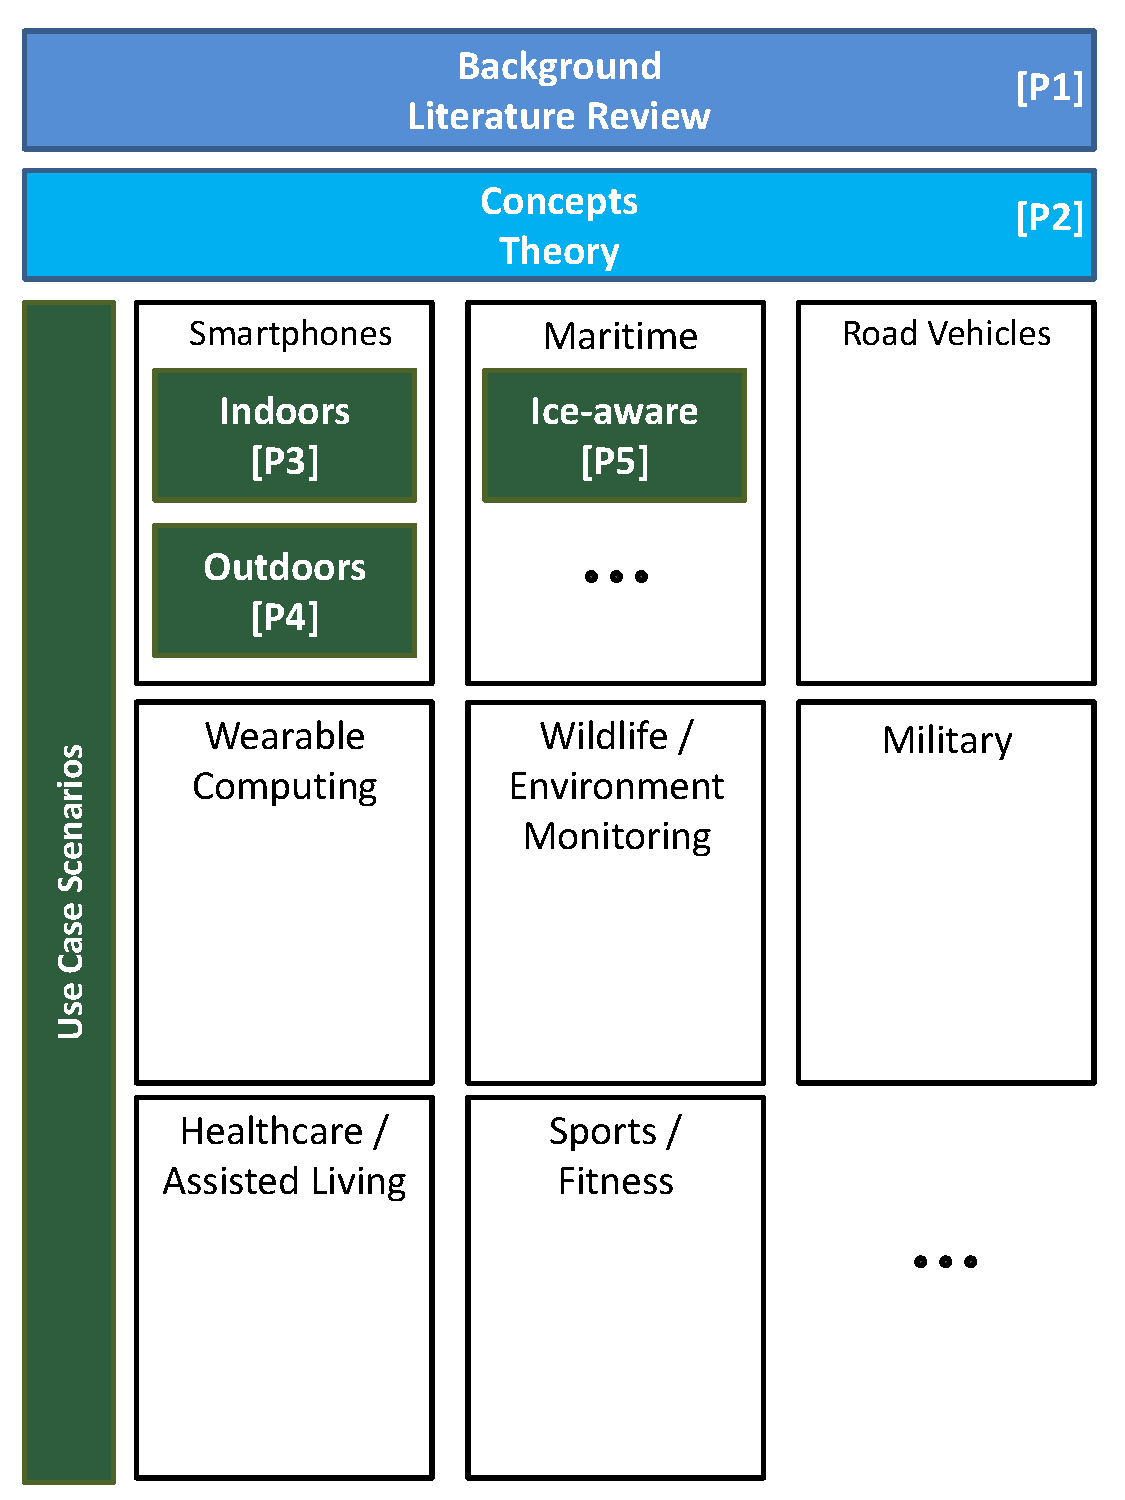
\includegraphics[width=1.0\textwidth]{Images/figChapter4}
  \end{center}
  \caption[Mapping of included publications to research areas]{Mapping of included publications to research areas. The additional empty boxes are intended to emphasize that many use case scenarios have yet to be explored. Further discussion on future use case scenarios can be found in Section~\ref{sec:future_applications}.}
  \label{fig:publication-chart}
\end{figure}

As Figure~\ref{fig:publication-chart} indicates, there are many potential use case scenarios that are not addressed in this thesis. There are, of course, many possible ways to categorize and sub-categorize the use cases, and this chart is not intended to be authoritative in this matter. The list is also not exhaustive. Our original research plan was to cover as many different use case scenarios as possible, but due to time constraints and project limitations, only two separate use case scenarios could be investigated (or three, if one considers [P3] and [P4] to cover separate use case scenarios). Our plans to cover additional use case scenarios will be discussed briefly in Chapter~\ref{ch:conclusions}.


\section{Author's Contributions to the Publications}
\label{sec:author_contributions}

This section outlines the main contributions of the author of this thesis to the included publications.

\textbf{[P1]:} The thesis author was the main author of this chapter, whereas the book co-author provided only editorial comments to a near-final draft. The thesis author conducted all the necessary background literature review and independently decided on the detailed contents of the chapter. The author also came up with the idea to use Hermagoras's ``seven elements of circumstance'' to organize and describe the different elements of context. The author also independently identified and collated the various Android Application Programming Interfaces (APIs) relevant to context awareness.

\textbf{[P2]:} The thesis author was the main author of this chapter, whereas the book co-author provided only editorial comments to a near-final draft. Similar to the case of [P1], the thesis author conducted all the necessary background literature review and independently decided on the detailed contents of the chapter. The author created all of the figures in the chapter and originated the concept of the ``context pyramid''. Finally, one of the main contributions of this chapter is the formulation and description (including figures) of rather complex mathematical concepts (e.g. \acrlong{svm}) in such a way that they are understandable to anyone with basic knowledge in algebra and probability.

\textbf{[P3]:} The thesis author was the second author of this publication, but the first author has affirmed in writing that the thesis author's contribution was roughly equal to that of the first author. The thesis author contributed equally to the design and implementation of the experiments. Implementation of the data collection application on a smartphone was primarily the responsibility of the thesis author. He also assisted in the analysis of the test results. In addition, he was the originator of the idea used for indoor-outdoor detection based on GPS signal-to-noise ratio and WiFi signal strength and implemented this method on a smartphone. The thesis author contributed to the development of the WiFi fingerprinting indoor positioning system and prepared the test environment by measuring and marking reference points and setting up additional WiFi access points. As stated earlier, he was the originator of the ``context pyramid'' concept, which is also described and employed in this paper. He was also the originator of the idea of using a graph-based grouping of the reference points. Lastly, he contributed to the preparation of the manuscript, including writing some sections and editing it in its entirety.

\textbf{[P4]:} The thesis author was the sole author of this publication and received assistance only in data collection, as well as general guidance from his supervisors. He also implemented all the necessary software used in the experiments, apart from the Weka software platform used in the data analysis. Some extensions to Weka, in terms of automating analysis and integrating Weka with Matlab, were also implemented by the author.

\textbf{[P5]:} The thesis author was the first author of this publication and was the originator of the idea of using a graph-based approach and the A* algorithm for ice-aware route optimization. He formulated the concept of combining a sea spatial model, ship maneuverability model, sea ice model, and ship performance model. In particular, the ship maneuverability model, which fixes the graph structure and discretizes the ship's maneuverability, was the thesis author's own invention. Furthermore, he implemented the optimization algorithm in Matlab, basing the implementation only roughly on an open source implementation.  The cost function was developed mainly by the thesis author, although various preliminary ideas were discussed together with the second author. The only parts of the method that were not implemented or provided by the thesis author were the resistive ship speed model, the ice data, and the historical ship data, all of which were provided by co-authors. Finally, the thesis author led the manuscript preparation, writing most sections, preparing all figures, and editing the manuscript in its entirety.